\chapter{Implementation} % Main chapter title
\label{chap:Implementation}

This chapter approaches the most technical component of this thesis. Here, it will be approached how the first version of the application was developed, considering both functional and non-functional requirements, defined in chapter \ref{chap:Requirements_Engineering}. Starting from how the code is structured in the different components, proceeding to the explanation of one of the main features of the project, the price calculation and how the code quality was measured. Finally, the application's user interfaces will be presented.

\section{Code Structure}
For the development of the project of this dissertation, the \gls{IDE} used was Visual Studio 2019. Each of the components identified in section \ref{sub:architectural-study} resulted in a solution in Visual Studio and, also, a different repository in the \gls{VCS}. In this case, the \gls{VCS} used was \textit{Git}.

\par

Inside the \gls{IDE}, the code was structured taking into account what was presented in section \ref{sec:internal-project-structure}. Each of the layers was mapped into a different \textit{Class Library} project. This allowed to have the code to be compiled separately which eases the management of dependencies between layers. After compilation, each project will result in a different \gls{DLL}. This allows for the compiled code to be used in different solutions by either having a direct reference to the compiled \gls{DLL}, or by creating a \textit{nuget} package and later installing it in the desired projects.
\par

The figure \ref{fig:vsProjects} presents the code structure on Visual Studio. For this example, the component used was the \textit{Order Management Service}.

\begin{figure}[!ht]
\centering
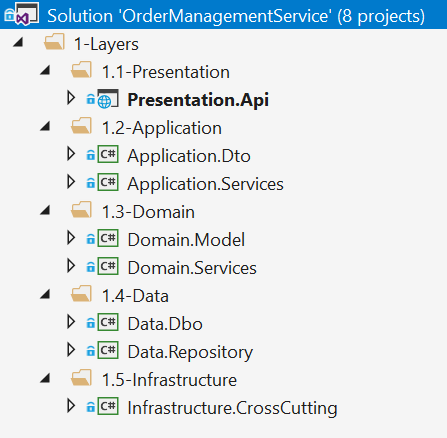
\includegraphics[width=0.8\textwidth,keepaspectratio]{chapters/Implementation/assets/vs-projects.PNG}
\caption[Code structure on Visual Studio]{Code structure on Visual Studio}
\label{fig:vsProjects}
\end{figure}

\section{Price Calculation}
The price calculation strategy is one of the most important components of an e-commerce website. It can be the thing that makes a customer come back to use the platform or, otherwise, it can be the thing that makes the customer to never come back. Furthermore, the calculation and breakdown of the price is also very important for law compliance. If, for example, the prices' \gls{VAT} parcel is not correctly calculated, the company may be paying less taxes than it should. This can result in fines that the company must pay, unnecessarily.

\par
 The price is an entity by itself rather than being a property of the service, as shown on figure \ref{fig:domainModel}. Each price has is immutable and have its own identifier. When an order is placed, this identifier is also persisted to keep a record of the price that was paid for each service. Also, this allows to have multiple prices for each service, if there is ever such a need. This is very useful for a use case where there are different prices for the same service, for example, with a \gls{VIP} customer segment, where customers in this segment have access to lower prices than a regular customer or have different prices for each country.

\par

On a technical level, when the user needs to update the price of a given service, the user makes that request to \textit{SnapTaks BO Management}, in the service details. This application uses BO API's endpoint to make the operation which afterwards makes a call to Pricing Service. This component is the one that contains all logic regarding prices and for that reason is where the logic for this operation is contained. The service will calculate the price, taking into account the \gls{VAT} and discount rates. If there is already a price in the database for the given service, that price will be disabled and the new price will be persisted as the price in use for that service.

\par

The sequence diagram in figure \ref{fig:priceUpdate} represents the update price flow between the several components of the platform.

\begin{figure}[ht]
\centering
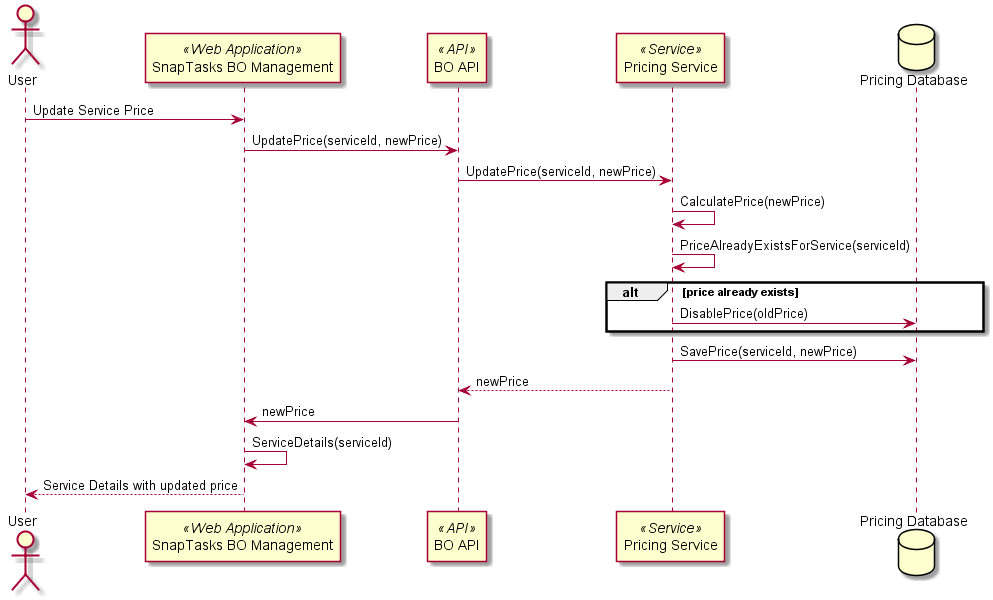
\includegraphics[width=\textwidth,keepaspectratio]{chapters/Implementation/assets/PriceUpdate.png}
\caption[Sequence diagram for price update]{Sequence diagram for price update}
\label{fig:priceUpdate}
\end{figure}

\par
The price composed by the \textbf{base price} and \textbf{final price}. The first one is the price that is defined by the \gls{SP}. This value does not take into account neither \gls{VAT} or discounts. These parcels are only accounted for in the final price, which is the price that will be paid by the customer for the given service. The formula below presents how the final price is calculated, using both \gls{VAT} and the discount rate.

\par

$$ finalPrice = basePrice * (1 + \frac{discountPercentage}{100}) * (1 + \frac{vatPercentage}{100})$$

\par

The discount is applied first, since it is to be applied to the price before taxes, otherwise the platform would be applying discounts over the tax value. Since the tax value is always to be paid to the taxable country, this would result in a wrong price calculation.

\par

In the case that the customer has a promocode, that promotion will be applied to the final order value, instead of being applied to each service price. The formula below presents how the total of an order is calculated.
\par
$$ total = ((\sum_{1}^{n} finalPrice) + logisticsFee) * (1 - \frac{promocodePercentage}{100})$$

\par
To reach this value, the final prices of all services are summed. Then, the logistics fee (value for the courier to do the transportation) is added to that value. Finally, if the customer used a promocode, that rate is reduced from the overall price.

\par

The platform will apply a commission model in order to retain profit. In a first phase, this commission has a flat rate of 10\% over the total of each order. However, this percentage may vary over the time and be different from service provider to service provider. 

$$ commission = total * ( \frac{commissionPercentage}{100})$$

\par

\section{Code Quality}
Many of the non-functional requirements identified in section \ref{sec:non-functional-requirements} can be measured by analyzing the code quality. This can provide an overview of requirements such as maintainability, resilience and performance.
\par
Code quality is the definition of code that is of good code (with a high-quality standard) and bad code (with a low-quality standard) \parencite{codeQuality}. The main problem with this definition remains on the concept of good and bad. Since this is very subjective, there is no golden rule to check if a given piece of code has the quality or not. 

\par

The desired quality for one team, organization, or even application, can be totally different from another. It all clings on what is the main objective of that code. While in more enterprise companies, that develop applications focused on the final user, need to have a code base that is maintainable, reusable and easily changed, companies that develop critical systems need their code to be resilient, failure proof and fast. These are non-functional requirements for the applications developed by such companies.

\par

To analyze the project's code quality, it was decided to use a code reviewing tool, in order to have an unbiased analysis. The chosen tool for this purpose was Codacy.

\par

Codacy is a static code analysis tool which aims to automate the code review process. It offers features to notify about security issues, code coverage, code duplication and code complexity \parencite{codacy}. After analyzing the code for potential problems, this tool assigns a grade to the project. 

\par

This grade ranges from \textbf{A} to \textbf{F}, being \textbf{A} the highest possible grade. This helps to have a better understanding of the quality of the project, taking into account issues of several categories:
\begin{itemize}
  \item Code Style
  \item Compatibility
  \item Error Prone
  \item Performance
  \item Security
  \item Unused Code
\end{itemize}

The calculation of the final grade is based on the number of found issues per \gls{KLOC}. Steve McConnell said in his book "Code Complete" that the industry average should be about 15 - 50 issues per \gls{KLOC}, when the code has some level of structured programming behind it \parencite{codeComplete}.

\par

With this, the objective for this project was to have a code base with a grade greater or equal to \textbf{B}. This objective was accomplished in every service of the SnapTasks platform. The figure \ref{fig:codacyGrade} presents the result of the code evaluation.


\begin{figure}[!ht]
\centering
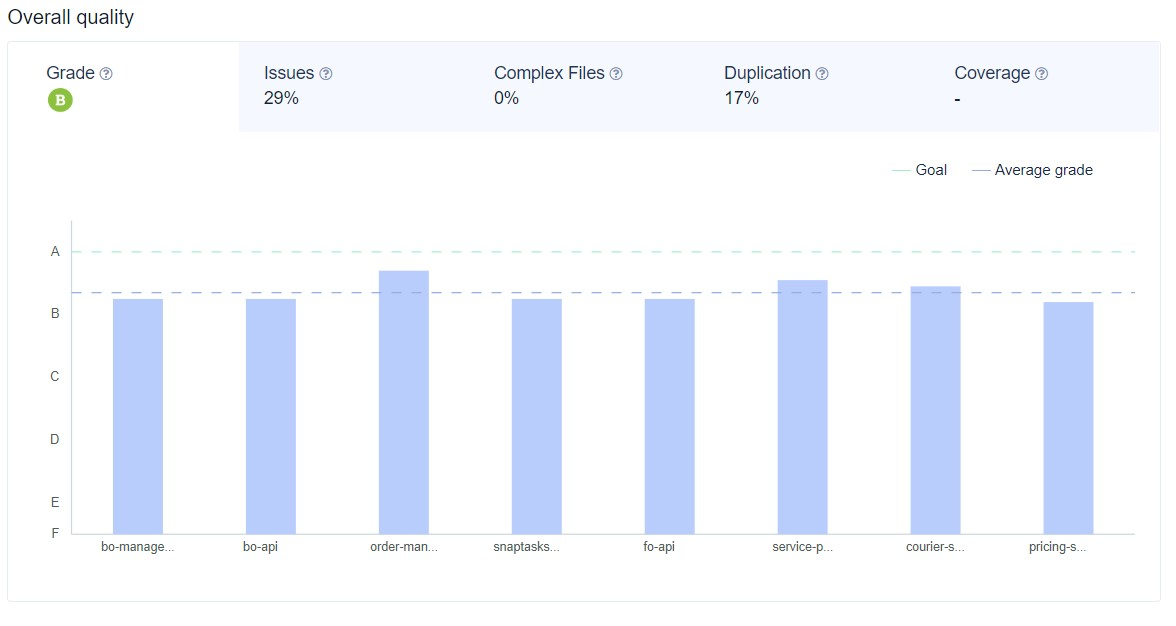
\includegraphics[width=\textwidth,keepaspectratio]{chapters/Implementation/assets/codacy-grade.jpg}
\caption[Codacy grade to SnapTasks projects]{Codacy grade to SnapTasks projects}
\label{fig:codacyGrade}
\end{figure}


\section{User Interfaces}
The user interface is one of the most critical topics for the success of a commercial software project. The user needs to find the application easy to use, attractive and consistent on all pages. The \gls{UI} is mostly important because it can turn visitors into buyers, as it facilitates the interactions between them and the system \parencite{uiDesignImportance}.
\par
The \gls{UI}s are also very important because it combines both the functional requirements of the system (what it will do) and the non-functional requirements (how it will be done), specified in sections \ref{sec:functional-requirements} and \ref{sec:non-functional-requirements}, respectively. The user interfaces can be considered the face of a given feature, since it is what the user will see, when interacting with the system.
\par
In this section, the most important pages of the two end-user applications (SnapTasks Portal, section \ref{sub:UI_SnaptasksPortal}, and SnapTasks BO Management, section \ref{sub:UI_BOManagement}) will be presented, grouped by the application they belong.


\subsection{SnapTasks Portal}
\label{sub:UI_SnaptasksPortal}
The SnapTasks Portal is the front-office application which the final customer will use. It provides features such as place order, check order history and check available services. Since this is the application where the customers will access, it is the one where there is a bigger need for a good \gls{UI}. 

\par

The most important pages of this application are the \textbf{Login Page}, the \textbf{Service Provider Listing Page}, the \textbf{Service Listing Page}, the \textbf{Service Display Page}, the \textbf{Checkout Page} and the \textbf{Order History Page}. These pages are described below.

\clearpage
\subsubsection{Login Page}

The login page is the page where the user will make the authentication, which will then allow him/her to access more actions, such as order history and place orders. The login may be done in two different ways: the first is to use an account that was previously created on the SnapTasks platform, using e-mail and password. the other is to use one external authentication service. Currently, there are two different authentication services: Facebook and Google. The figure \ref{fig:snaptasksLogin} presents the \gls{UI} of the login page.

\begin{figure}[ht]
\centering
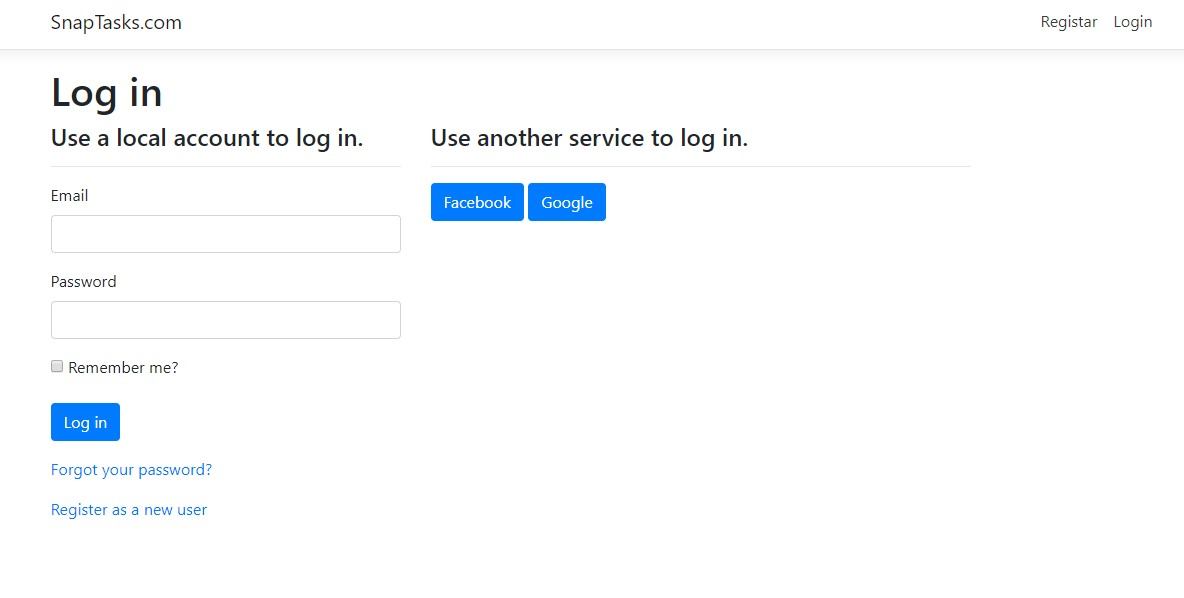
\includegraphics[width=0.65\textwidth,keepaspectratio]{chapters/Implementation/assets/snaptasks-login.jpg}
\caption[SnapTasks login page]{SnapTasks login page}
\label{fig:snaptasksLogin}
\end{figure}


\subsubsection{Service Provider Listing Page (SPLP)}

The \gls{SPLP} is one of the most important pages in the SnapTasks Portal, since it serves as the home page of the application. The main purpose of this page is to present the service providers available on the platform. To that responsibility are added the ones of a home page, which are mainly to catch the attention of the end user and make it appealing to browse the website. The figure \ref{fig:snaptasksSPLP} presents the \gls{GUI} of this page.

\begin{figure}[ht]
\centering
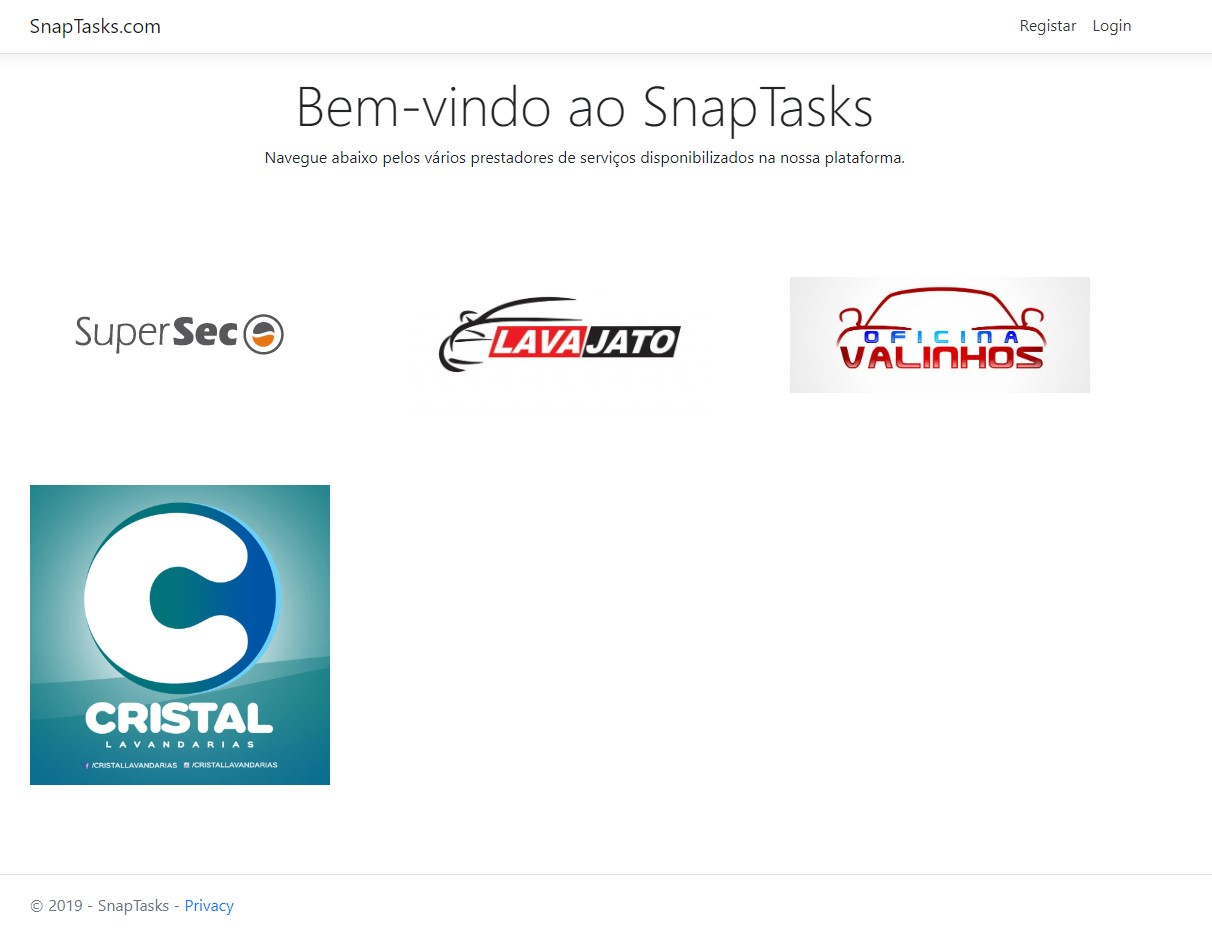
\includegraphics[width=0.65\textwidth,keepaspectratio]{chapters/Implementation/assets/snaptasks-splp.jpg}
\caption[SnapTasks service provider listing page]{SnapTasks service provider listing page}
\label{fig:snaptasksSPLP}
\end{figure}

\clearpage
\subsubsection{Service Listing Page (SLP)}
\label{sub:service-listing-page}
The \gls{SLP} is accessed when the user selects a service provider in the \gls{SPLP}. This page presents the list of services that are provided by the selected \gls{SP}. Besides the name of the service, it also presents a description of the service and its price. The figure \ref{fig:serviceListingPage} presents the \gls{UI} of this page.

\begin{figure}[!ht]
\centering
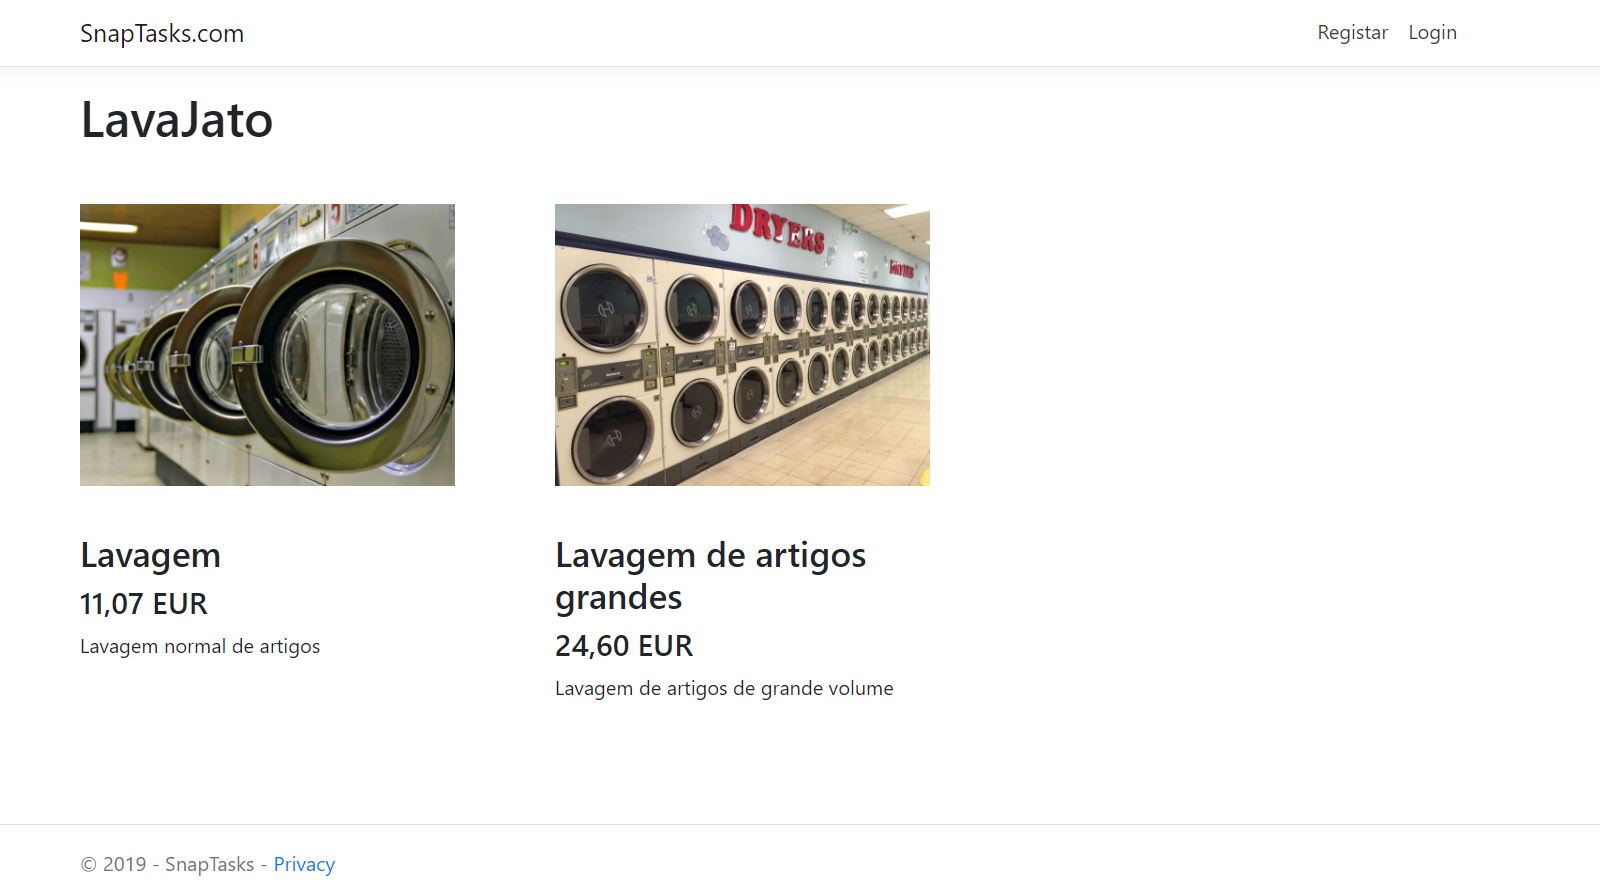
\includegraphics[width=0.9\textwidth,keepaspectratio]{chapters/Implementation/assets/snaptasks-slp.PNG}
\caption[Service Listing Page of a Service Provider]{Service Listing Page of a Service Provider}
\label{fig:serviceListingPage}
\end{figure}


\subsubsection{Service Display Page (SDP)}
When the user selects a service in the \gls{SLP}, he/she is redirected to the \gls{SDP}. This page has as its main purpose to display the details of the selected service. It provides information such as a more detailed description, the base price, the \gls{VAT} and discounts (if any) and the final price. This page also provides the option for the user to place an order for that service. The \gls{UI} of that page is presented in figure \ref{fig:snaptasksSDP}.

\begin{figure}[ht]
\centering
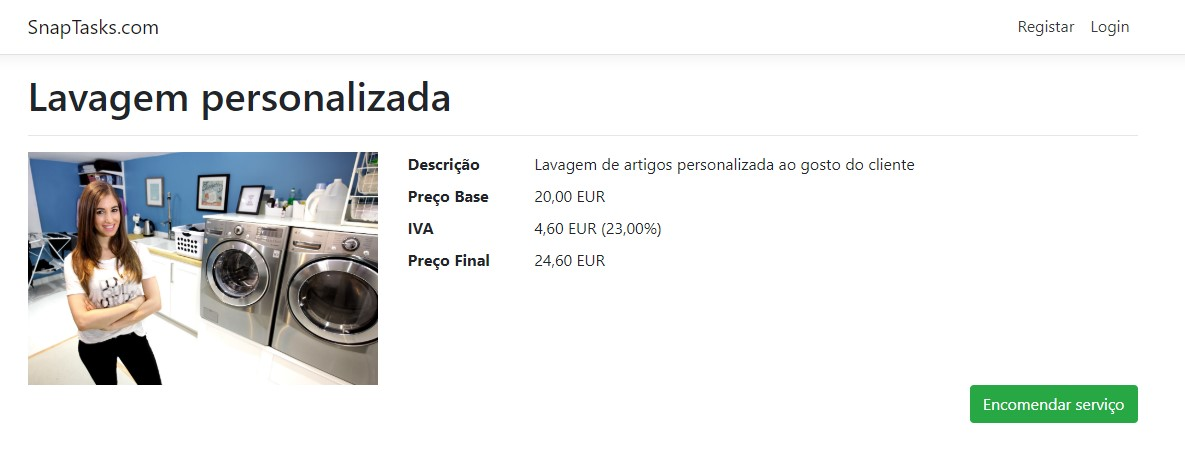
\includegraphics[width=0.9\textwidth,keepaspectratio]{chapters/Implementation/assets/snaptasks-sdp.jpg}
\caption[SnapTasks service display page]{SnapTasks service display page}
\label{fig:snaptasksSDP}
\end{figure}

\clearpage
\subsubsection{Checkout Page}
The checkout page is the page where the customer places an order. It provides the information of the selected service, informs the total value of the order and asks for the information needed to fulfill the order (date of pickup, billing and pickup address and payment information).
\par

For the payment processing, SnapTasks integrates with a third-party payment provider, Stripe, that processes the payments in a secure way. Stripe also provides tools for testing purposes, as several test credit cards.

\par

This page is presented in figure \ref{fig:snaptasksCheckout}.
\begin{figure}[ht]
\centering
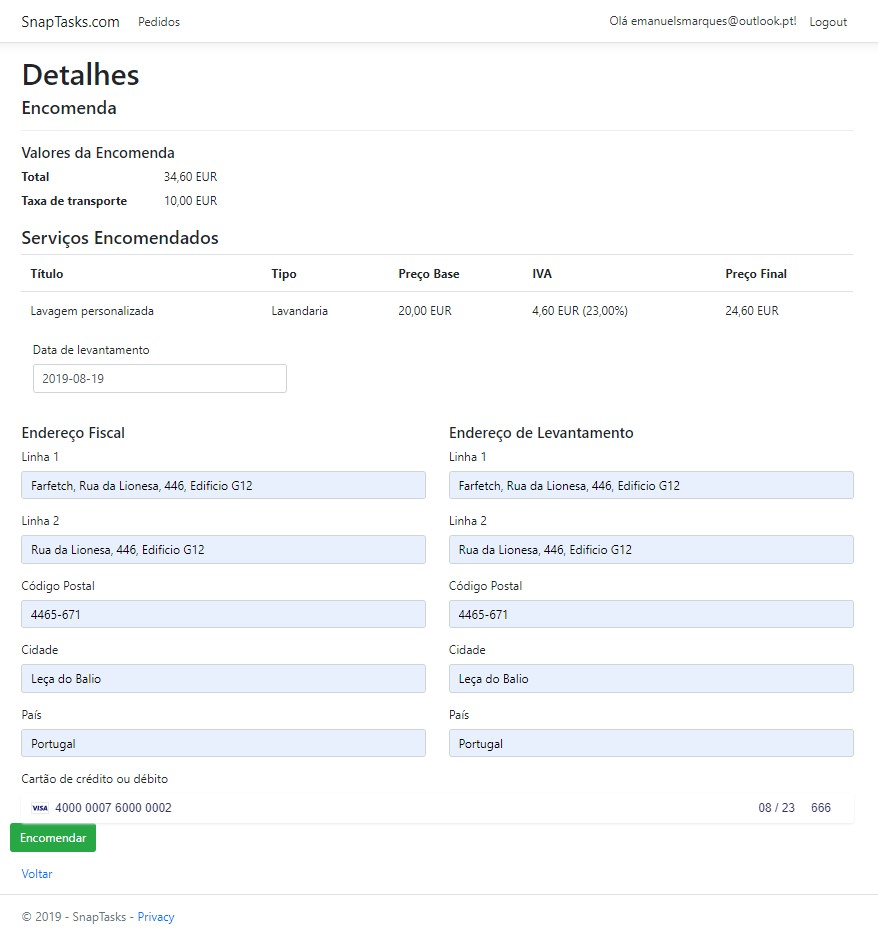
\includegraphics[width=\textwidth,keepaspectratio]{chapters/Implementation/assets/snaptasks-checkout.jpg}
\caption[SnapTasks checkout page]{SnapTasks checkout page}
\label{fig:snaptasksCheckout}
\end{figure}


\subsubsection{Order Details Page}
To access further information regarding an order, the user can open the details, in the order history page. This will redirect the user to the order details page. This page presents all the relevant information that concerns the selected order. The page presents the ordered services, the billing and pickup address, the values of the order (both final price and total. Check how these fields are calculated in section \ref{sec:Implementation_DomainModel}), the order status and the pickup date.

\par

The \gls{UI} of this page is presented in figure \ref{fig:snaptasksOrderDetails}.

\begin{figure}[ht]
\centering
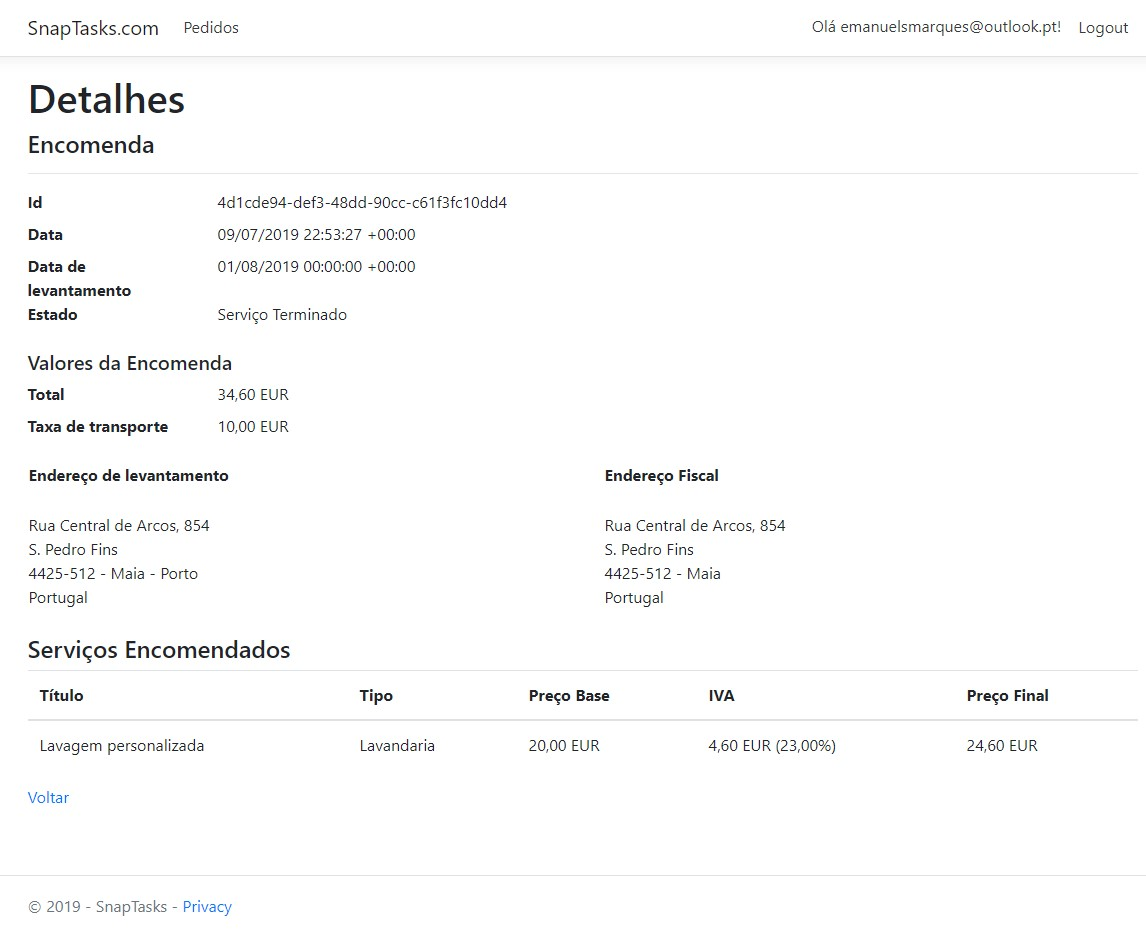
\includegraphics[width=\textwidth,keepaspectratio]{chapters/Implementation/assets/snaptasks-orderDetails.jpg}
\caption[SnapTasks order details page]{SnapTasks order details page}
\label{fig:snaptasksOrderDetails}
\end{figure}


\clearpage
\subsubsection{Order History Page}
The order history presents the customer all the orders he/she had placed in the past. This page shows basic information about the order, such as the identifier, the creation date, the total value and the current status. With this page, it is possible to have an awareness of all the orders that were placed and their status. The figure \ref{fig:snaptasksOrderHistory} presents the \gls{UI} of this page.

\begin{figure}[ht]
\centering
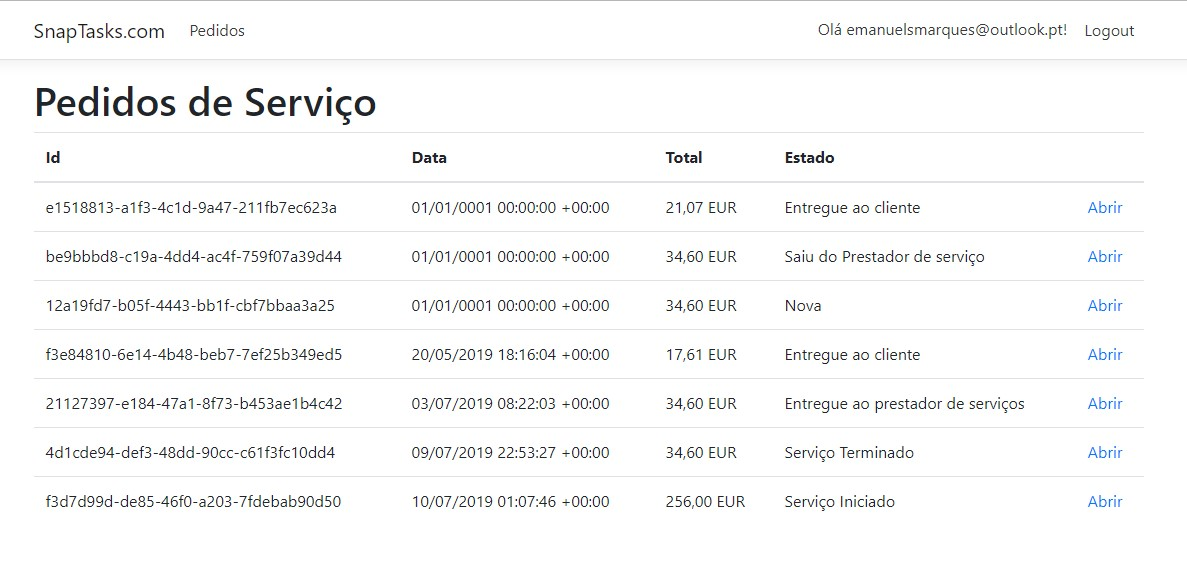
\includegraphics[width=\textwidth,keepaspectratio]{chapters/Implementation/assets/snaptasks-orderhistory.jpg}
\caption[SnapTasks order history page]{SnapTasks order history page}
\label{fig:snaptasksOrderHistory}
\end{figure}

\clearpage

\clearpage
\subsection{SnapTasks Back-Office Management}
\label{sub:UI_BOManagement}
SnapTasks BO Management is an application whose purpose is to provide back-office and management tools. This application is designed to be used mostly by the operations teams who have the responsibility to manage the service providers, the couriers and the orders.
\par
Since this application is not to be used by final customers, the \gls{UI} that is used is not as critical as in the SnapTasks Portal. However, it is still very important that the use of features is intuitive and easy to learn, since the less time something takes to be done, the cheaper it will be.

\par

The pages of this application are grouped into three main categories: 

\begin{itemize}
    \item \textbf{Service Provider Management Pages}, which are the pages where the \gls{SP}s and their services will be listed, created, edited and disabled;
    \item \textbf{Order Management Pages}, where the placed orders can be listed, accessed and processed;
    \item \textbf{Courier Management Pages}, whose pages have the purpose of creation, edit and disable couriers.
\end{itemize}

These pages are further detailed and presented in the next sections.


\subsubsection{Service Provider Management Pages}

The Service Provider Management pages are the group of pages that provide tools to manage the service providers and their services. It is possible to create, disable, and edit both the service providers and its services. For the last case, it is also possible to update the price of a service. These pages can be accessed by the administrators of the platform, who can create and edit any \gls{SP} and its services, and by the service provider's account, who can just edit their information and services. 

\par

The figure \ref{fig:snaptasksSPList} presents the page that lists the current active service providers in the platform and the figure \ref{fig:snaptasksSPDetails} shows the details of a service provider, and which services it provides.

\begin{figure}[!ht]
\centering
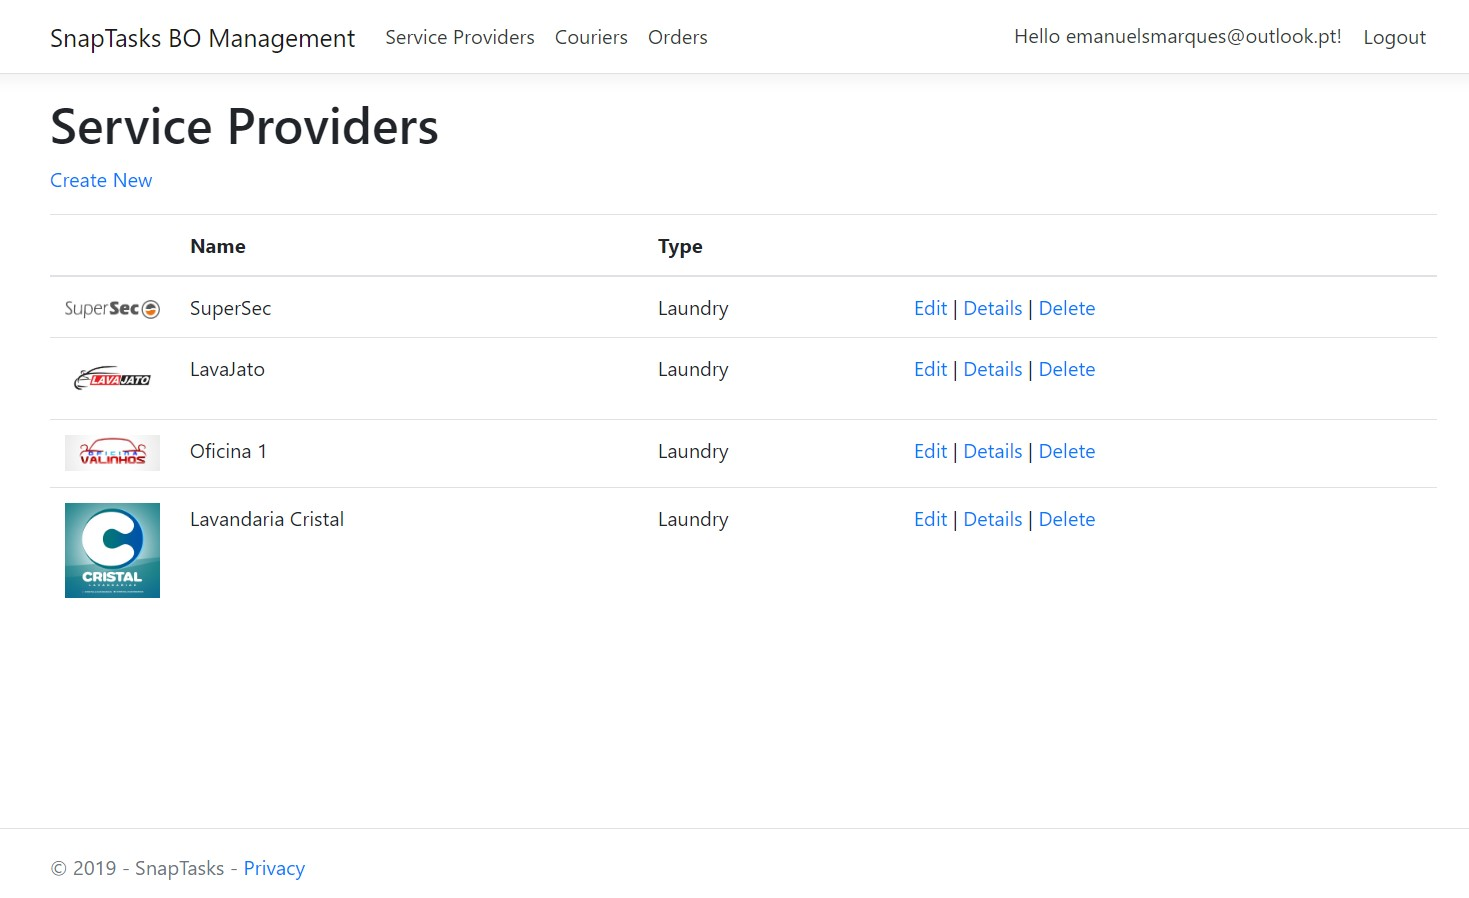
\includegraphics[width=0.7\textwidth,keepaspectratio]{chapters/Implementation/assets/snaptasks-bo-listSP.jpg}
\caption[List of service providers page]{List of service providers page}
\label{fig:snaptasksSPList}
\end{figure}

\begin{figure}[!ht]
\centering
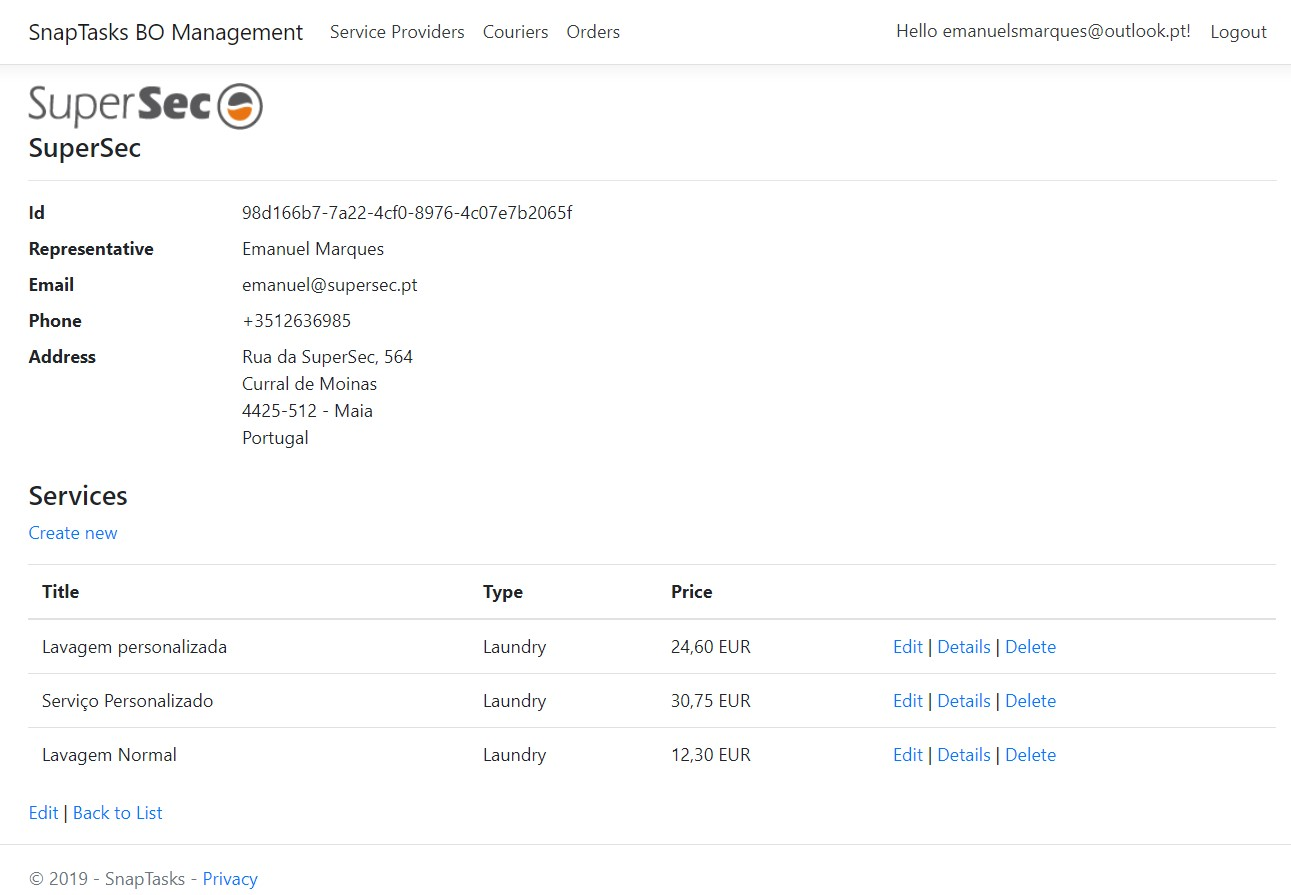
\includegraphics[width=0.8\textwidth,keepaspectratio]{chapters/Implementation/assets/snaptasks-bo-detailsSP.jpg}
\caption[Service Provider details page]{Service Provider details page}
\label{fig:snaptasksSPDetails}
\end{figure}


\subsubsection{Courier Management Pages}
Similarly to the previous pages, this group contains the features to create, edit and disable couriers. This is essentially an administration feature since only platform administrators have access to it.
\par
The figure \ref{fig:snaptasksCourierList} presents the page that lists all the available couriers.

\begin{figure}[ht]
\centering
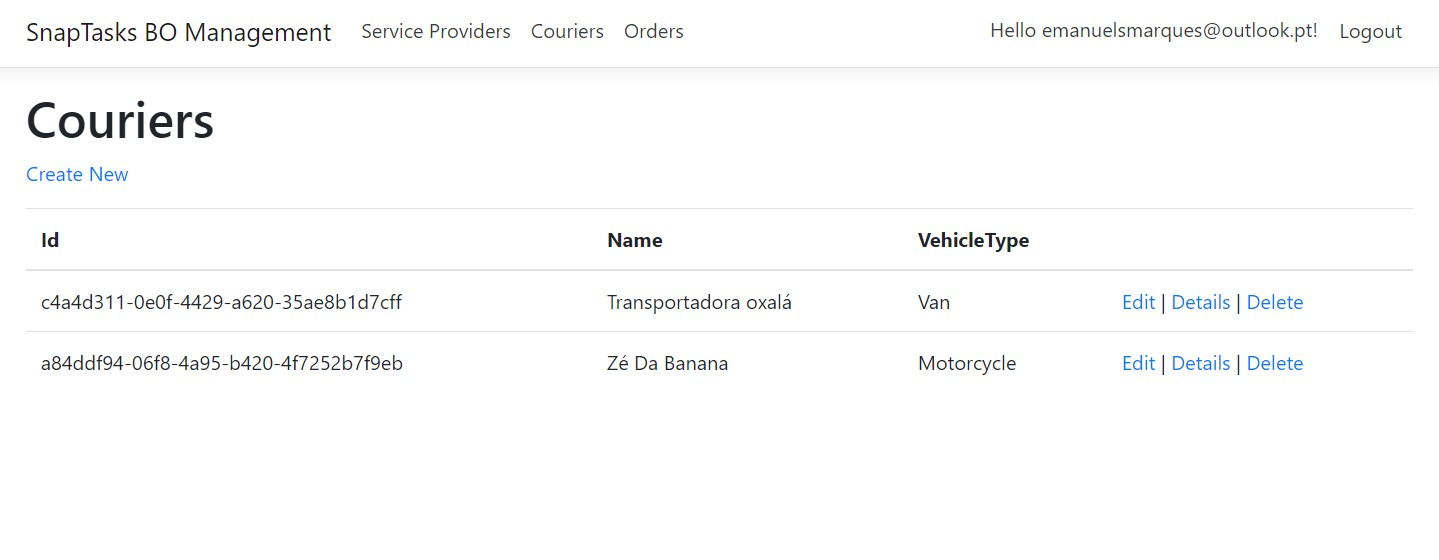
\includegraphics[width=\textwidth,keepaspectratio]{chapters/Implementation/assets/snaptasks-bo-listCouriers.jpg}
\caption[Courier list page]{Courier list page}
\label{fig:snaptasksCourierList}
\end{figure}


\subsubsection{Order Management Pages}

The order management pages are the pages where order information will be available and order processing features (like changing step, or courier assignment) will be available. Here is also possible to view the details of a given order and check the order history.

\par

The figure \ref{fig:snaptasksOrderList} presents the page that lists the placed orders to be processed in the platform and the ones that were already processed. The figure \ref{fig:snaptasksOrderDetailsBO} shows the details of a given order.

\begin{figure}[!ht]
\centering
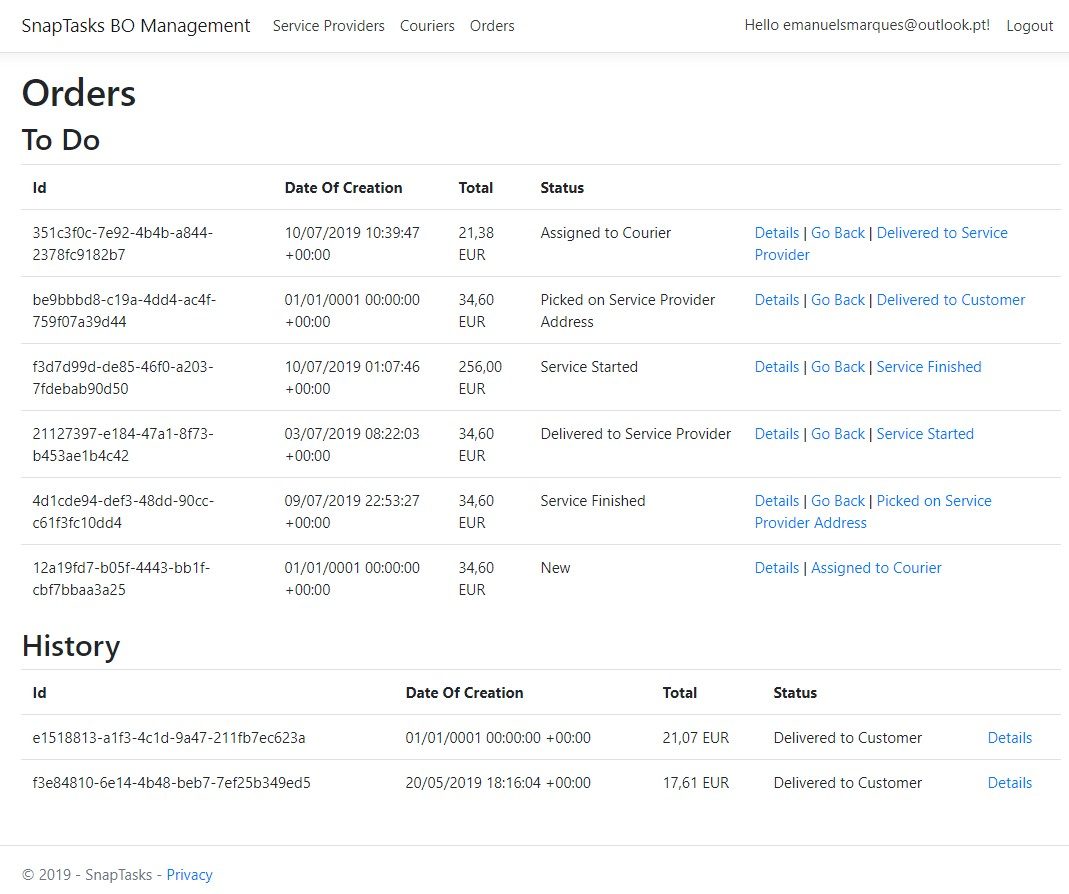
\includegraphics[width=0.8\textwidth,keepaspectratio]{chapters/Implementation/assets/snaptasks-bo-todo.jpg}
\caption[Order Processing Page]{Order Processing Page}
\label{fig:snaptasksOrderList}
\end{figure}

\begin{figure}[!ht]
\centering
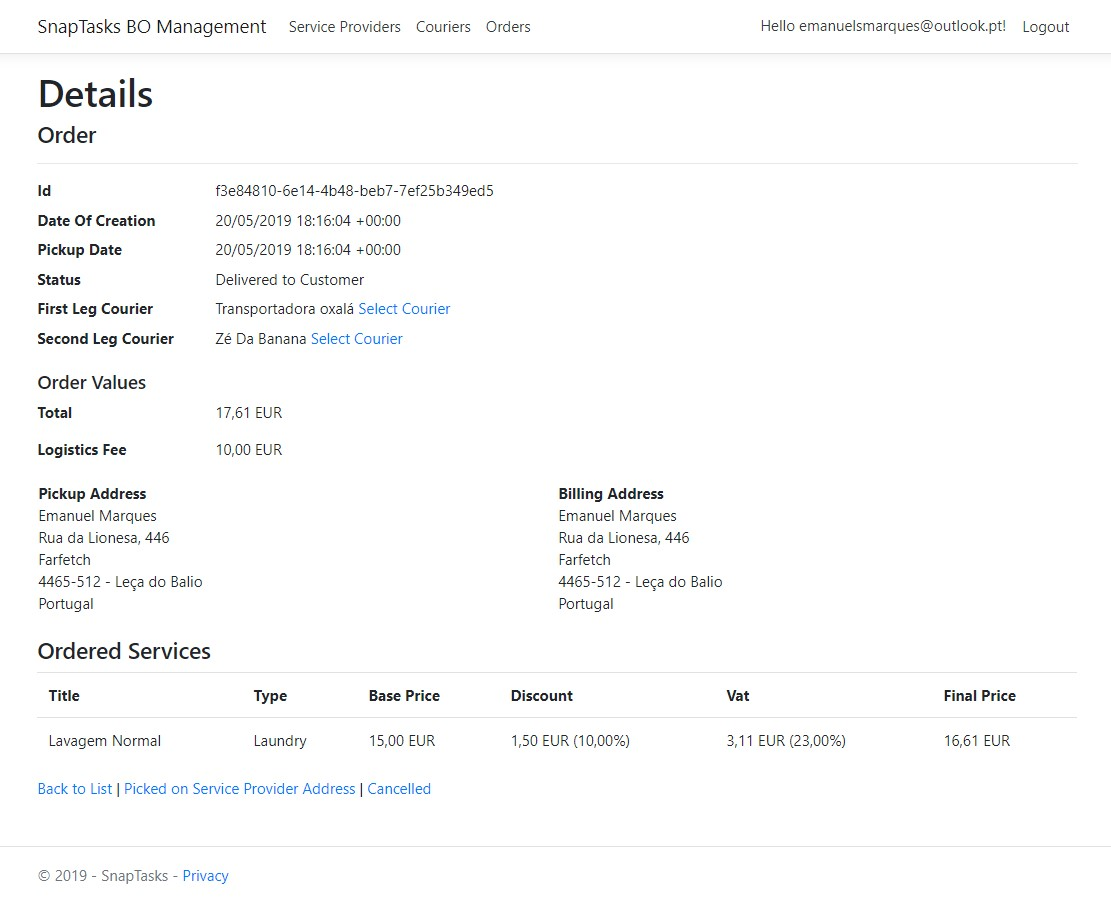
\includegraphics[width=0.8\textwidth,keepaspectratio]{chapters/Implementation/assets/snaptasks-bo-orderDetails.jpg}
\caption[Order details page]{Order details page}
\label{fig:snaptasksOrderDetailsBO}
\end{figure}


